\documentclass{article}

\usepackage{spconf}

%\interdisplaylinepenalty=2500

\usepackage{graphicx}
\graphicspath{{../Figures/}}

\usepackage{amsmath,amssymb,amsfonts}
\usepackage{upgreek}
\usepackage[retainorgcmds]{IEEEtrantools}

\usepackage{hyperref}
%\usepackage[capitalize]{cleveref}

%\usepackage{fancyhdr}
%\pagestyle{fancy}
%\fancyhead{}
%\fancyfoot[C]{Distribution A: Approved for public release; Distribution unlimited}
%\renewcommand{\headrulewidth}{0pt}


\usepackage{mathfont_shortcuts}
\usepackage{PhDmath}


%\DeclareMathOperator*{\argmin}{arg\,min}
%\DeclareMathOperator*{\argmax}{arg\,max}
%\newcommand{\inprob}{\overset{p}{\to}}
%
%
%\DeclareMathOperator{\Rbbgeq}{\mathbb{R}_{\geq 0}}
%\DeclareMathOperator{\Zbbgeq}{\mathbb{Z}_{\geq 0}}
%
%\DeclareMathOperator{\Dir}{\mathrm{Dir}}
%\DeclareMathOperator{\DM}{\mathrm{DM}}
%\DeclareMathOperator{\Multi}{\mathrm{Multi}}
%\DeclareMathOperator{\Bi}{\mathrm{Bi}}
%\DeclareMathOperator{\DP}{\mathrm{DP}}
%\DeclareMathOperator{\DMP}{\mathrm{DMP}}
%\DeclareMathOperator{\Emp}{\mathrm{Emp}}
%\DeclareMathOperator{\DE}{\mathrm{DE}}
%\DeclareMathOperator{\EP}{\mathrm{EP}}
%\DeclareMathOperator{\DEP}{\mathrm{DEP}}
%
%\DeclareMathOperator{\thetam}{\theta_\text{m}}
%\DeclareMathOperator{\upthetam}{\uptheta_\text{m}}
%\DeclareMathOperator{\thetac}{\theta_\text{c}}
%\DeclareMathOperator{\upthetac}{\uptheta_\text{c}}
%
%\DeclareMathOperator{\psim}{\psi_\text{m}}
%\DeclareMathOperator{\Psim}{\Psi_\text{m}}
%\DeclareMathOperator{\uppsim}{\uppsi_\text{m}}
%\DeclareMathOperator{\Uppsim}{\Uppsi_\text{m}}
%\DeclareMathOperator{\psic}{\psi_\text{c}}
%\DeclareMathOperator{\Psic}{\Psi_\text{c}}
%\DeclareMathOperator{\uppsic}{\uppsi_\text{c}}
%\DeclareMathOperator{\Uppsic}{\Uppsi_\text{c}}
%
%\DeclareMathOperator{\alpham}{\alpha_\text{m}}
%\DeclareMathOperator{\alphac}{\alpha_\text{c}}



\title{Bayesian Learning for Regression using Dirichlet Prior Distributions of Varying Localization}

%\name{Anonymous\thanks{Anonymous.}}
%\address{Anonymous}

\twoauthors
  {Paul Rademacher}
	{U.S. Naval Research Laboratory\\Radar Division\\Washington, DC 20375, USA\\paul.rademacher@nrl.navy.mil}
  {Milo\v{s} Doroslova\v{c}ki}
	{The George Washington University\\Department of Electrical and Computer Engineering\\Washington, DC 20052, USA\\
   doroslov@gwu.edu}



\begin{document}

\maketitle


\begin{abstract}
When taking a Bayesian approach to machine learning applications, the performance of the learned function strongly depends on how well the prior distribution selected by the designer matches the true data-generating model. Dirichlet priors have a number of desirable properties -- they result in closed-form posterior distributions given independent training data, have full support over the space of data probability distributions, and can be maximally informative or non-informative depending on their localization parameter. This paper assumes a Dirichlet prior and details the predictive distributions that characterize unobservable random quantities given observed data. The results are then applied to the most common loss function for regression, the squared error loss. The optimal Bayes estimator and the resultant risk trends are presented for different prior localizations, demonstrating a bias/variance trade-off. 
\end{abstract}

\begin{keywords}
Bayesian learning, machine learning, regression, estimation, Dirichlet distribution, bias, variance, predictive distribution
\end{keywords}


\section{Introduction}

The success or failure of Bayesian learning methods hinges on how well the prior knowledge imparted by the designer matches reality. The chosen prior distribution over the set of data-generating probability distributions reflects the user's confidence that different models are responsible for generating the observed/unobserved random elements. If a highly localized, ``informative" prior that strongly weights the actual data model is chosen, low risk learning functions are possible even with limited training data; however, if the localized prior is poorly selected, a good solution may not be achieved. Conversely, a non-informative prior provides fast adaptation during training and can be suitable for a variety of problems; if data is limited, however, the learning function may not deliver satisfactory performance.

This work assumes that the observed and unobserved data elements are jointly characterized by a Dirichlet prior. The class of Dirichlet probability density functions (PDF) has the desirable property of full support, guaranteeing consistent estimation of the true data-generating distribution; it also leads to a closed-form posterior distribution for independently and identically distributed (i.i.d.) data \cite{ferguson}. Furthermore, control of the Dirichlet parameters enables both minimally and maximally informative priors, providing a wide range of learning solutions.

After motivating the Bayesian perspective and using the Dirichlet prior to generate the predictive distribution, the results will be applied to the squared error loss function. The optimal Bayes estimator and the achieved risk will be presented. Results will demonstrate a bias/variance risk trade-off dependent on prior parameterization, exemplifying the balance between prior knowledge and data utilization. Comparison with a classical Bayesian regressor will be performed.


\section{Objective}

Consider an observable scalar random variable $\xrm \in \Xcal \subset \Rbb$ and unobservable scalar random variable $\yrm \in \Ycal \subset \Rbb$ which are jointly distributed according to an unknown probability mass function (PMF), $\theta \in \Pcal(\Ycal \times \Xcal) \equiv \Big\{ \theta \in {\Rbb_{\geq 0}}^{\Ycal \times \Xcal}: \sum_{y,x} \theta(y,x) = 1 \Big\}$, such that $\Prm_{\yrm,\xrm | \uptheta}(y,x | \theta) = \theta(y,x)$. The space $\Pcal(\cdot)$ is the set of probability distributions over the argument set.

Also observed is a random sequence of $N$ samples drawn from the model $\theta$, denoted $\Drm \in \Dcal = \{\Ycal \times \Xcal\}^N$. The $N$ data pairs are identically distributed as $\Prm_{\Drm_n | \uptheta}(y,x | \theta) = \theta(y,x)$ for $n = 1,\ldots,N$ and are conditionally independent from one another and from the novel pair $(\yrm,\xrm)$.

The regression objective is to design a learning function $f: \Dcal \mapsto \Rbb^{\Xcal}$ which uses the training data to select an estimator from the set of functions $\Xcal \mapsto \Rbb$. The metric guiding the design is the squared error loss function $\Lcal: \Rbb \times \Ycal \mapsto \Rbb_{\geq 0}$, defined as $\Lcal(y',y) = (y'-y)^2$. The expected loss, or ``risk'', is defined as
\begin{IEEEeqnarray}{L} \label{eq:risk_cond}
\Rcal_{\Theta}(f ; \uptheta) = \Erm_{\Drm | \uptheta} \bigg[ \Erm_{\yrm,\xrm | \uptheta} \Big[ \big( f(\xrm;\Drm)-\yrm \big)^2 \Big] \bigg] \\
\quad = \Erm_{\xrm | \uptheta} \left[ \Sigma_{\yrm | \xrm,\uptheta} \right] + \Erm_{\xrm,\Drm | \uptheta} \Big[ \big( f(\xrm;\Drm) - \mu_{\yrm | \xrm,\uptheta} \big)^2 \Big] \nonumber \;,
\end{IEEEeqnarray}
where $\mu$ and $\Sigma$ are the mean and covariance functions, respectively.

%PGR: quadratic min??

If the model $\theta$ were known, the ``clairvoyant'' \cite{kay-det} estimate would be $f_{\Theta}(\xrm;\uptheta) = \mu_{\yrm | \xrm,\uptheta}$, and the minimum risk $\Rcal_{\Theta}^*(\uptheta) = \Erm_{\xrm | \uptheta} \left[ \Sigma_{\yrm | \xrm,\uptheta} \right]$ would be achieved. Sub-optimal learners induce excess risk $\Rcal_{\Theta, \mathrm{ex}}(f ; \uptheta) \equiv \Rcal_{\Theta}(f ; \uptheta) - \Rcal_{\Theta}^*(\uptheta)$ due to model uncertainty.

As the model $\theta$ is not observed, $\Rcal_{\Theta}$ is not a feasible objective function for optimization. If the designer selects a PDF $\prm_{\uptheta}$, the Bayes risk is formulated as
\begin{IEEEeqnarray}{rCl} \label{eq:risk}
\Rcal(f; \prm_{\uptheta}) & = & \Erm_{\uptheta}\big[ \Rcal_{\Theta}(f ; \uptheta) \big] \nonumber \\
& \equiv & \Erm_{\xrm,\Drm} \bigg[ \Erm_{\yrm | \xrm,\Drm} \Big[ \big( f(\xrm;\Drm)-\yrm \big)^2 \Big] \bigg] 
\end{IEEEeqnarray}
and $\yrm$, $\xrm$, and $\Drm$ are treated as jointly distributed random variables. The optimal Bayesian estimate is expressed as
\begin{IEEEeqnarray}{rCl} \label{eq:f_opt_xD}
f^*(\xrm;\Drm) & = & \argmin_{y' \in \Rbb} \Erm_{\yrm | \xrm,\Drm}\big[ (y'-\yrm)^2 \big] = \mu_{\yrm | \xrm,\Drm} \;,
\end{IEEEeqnarray}
where the dependency of $f^*$ on the prior $\prm_{\uptheta}$ (through $\Prm_{\yrm | \xrm,\Drm}$) is suppressed for brevity.







\section{Probability Distributions}


\subsection{Dirichlet Model Process} \label{sec:P_theta}

The Dirichlet prior PDF for the model random process $\uptheta \in \Theta$ is \cite{bishop}
\begin{IEEEeqnarray}{rCl}
\prm_{\uptheta}(\theta) & = & \beta(\alpha_0 \alpha)^{-1} \prod_{y \in \Ycal} \prod_{x \in \Xcal} \theta(y,x)^{\alpha_0 \alpha(y,x) - 1} \nonumber \\
& \equiv & \Dir(\theta; \alpha_0,\alpha) \;,
\end{IEEEeqnarray}
where $\beta$ is the multivariate beta function, and the localization parameter $\alpha_0 \in \Rbb^+$ and mean $\alpha \in \Pcal(\Ycal \times \Xcal) \cap {\Rbb^+}^{\Ycal \times \Xcal}$ are introduced. Note that as $\alpha_0 \to \infty$, $\uptheta \inprob \alpha$ and thus the PDF tends to a maximally informative prior $\prm_{\uptheta} \to \delta(\cdot - \alpha)$, where $\delta$ is the Dirac delta function over $\Pcal(\Ycal \times \Xcal)$.



\subsubsection{Marginal and Conditional Models} \label{sec:P_theta_mc}

An alternative representation is implemented via the bijection $\uptheta \Leftrightarrow (\upthetam,\upthetac)$, where the marginal distribution $\upthetam \equiv \sum_{y \in \Ycal} \uptheta(y,\cdot) \in \Pcal(\Xcal)$ and the conditional distributions $\upthetac(x) \equiv \uptheta(\cdot,x) / \upthetam(x) \in \Pcal(\Ycal)$ for all $x \in \Xcal$. 

By the aggregation property \cite{ferguson}, $\upthetam \sim \Dir(\alpha_0,\alpham)$ is a Dirichlet random process parameterized by localization $\alpha_0$ and mean $\alpham \equiv \sum_{y \in \Ycal} \alpha(y,\cdot)$. Also, it can be shown that the predictive models $\upthetac(x) \sim \Dir\big(\alpha_0 \alpham(x),\alphac(x)\big)$ are independent Dirichlet processes with mean functions $\alphac(x) \equiv \alpha(\cdot,x) / \alpham(x)$; they are each independent of $\upthetam$, as well. 







\subsection{Training Data and the Empirical Statistic}

Using the i.i.d. assumption, the distribution of the training data $\Drm$ conditioned on the model can be formulated as
\begin{IEEEeqnarray}{rCl}
\Prm_{\Drm | \uptheta}\big( D | \theta \big) & = & \left( \prod_{y \in \Ycal} \prod_{x \in \Xcal} \theta(y,x)^{\Psi(y,x;D)} \right)^N \;,
\end{IEEEeqnarray}
where the dependency on the training data $\Drm$ is expressed though a transform function $\Psi : \Dcal \mapsto \Uppsi \subset \Pcal(\Ycal \times \Xcal)$ defined as $\Psi(y,x;D) = N^{-1} \sum_{n=1}^N \delta \big[ (y,x),D_n \big]$. 


%As the conditional distribution $\Prm_{\Drm | \uptheta}$ is of exponential form, it can be readily shown that the marginal distribution of the training data is \cite{minka-multi}
%\begin{IEEEeqnarray}{rCl}
%\Prm_{\Drm}(D) & = & \beta(\alpha)^{-1} \beta \left(  \alpha + \bar{N}(D) \right) \;.
%\end{IEEEeqnarray}


This transform produces the empirical distribution of the training data $\Drm$. Since the distribution $\Prm_{\Drm | \uptheta}$ depends on the training data only via $\Psi$, $\Psi(\Drm)$ is a sufficient statistic \cite{bernardo} for the model $\uptheta$. As such, the analysis is performed using a new random process $\uppsi \equiv \Psi(\Drm) \in \Uppsi$, noting that $\Prm_{\yrm | \xrm,\Drm}(x,D) = \Prm_{\yrm | \xrm,\uppsi}\big( x,\Psi(D) \big)$. 

Note that $\Uppsi$ is a sampling of the distribution space $\Pcal(\Ycal \times \Xcal)$ with cardinality $|\Uppsi| = \Mcal\big( (N,|\Ycal||\Xcal|-1) \big)$, where $\Mcal$ is the multinomial coefficient; this can be shown using the stars-and-bars method \cite{feller}. Additionally, $|\Uppsi| \leq |\Dcal| = \big( |\Ycal| |\Xcal| \big)^N$ and thus the sufficient statistic efficiently represents the information in the training data. 

The conditional distribution of the transformed process is
\begin{IEEEeqnarray}{rCl}
\Prm_{\uppsi | \uptheta}(\psi | \theta) & = & \Mcal(N \psi) \left( \prod_{y \in \Ycal} \prod_{x \in \Xcal} \theta(y,x)^{\psi(y,x)} \right)^N \nonumber \\
& \equiv & \Emp\big( \psi;N,\theta \big) \;,
\end{IEEEeqnarray}
an empirical PMF. As $\uppsi | \uptheta$ is equivalent to a normalized multinomial random process \cite{minka-multi}, the mean and covariance functions are $\mu_{\uppsi | \uptheta} = \uptheta$ and
\begin{IEEEeqnarray}{L}
\Sigma_{\uppsi | \uptheta}(y,x,y',x' | \theta) \\
\qquad = \frac{1}{N} \theta(y,x) \big( \delta[y,y'] \delta[x,x'] - \theta(y',x') \big) \nonumber \;.
\end{IEEEeqnarray}
Note that as $N \to \infty$, the process converges to $\uppsi | \uptheta \inprob \uptheta$.



\subsubsection{Marginal and Conditional Data Statistics} \label{sec:P_psi-theta_mc}

The empirical process can also be decomposed into marginal and conditional empirical processes via a bijection $\uppsi \Leftrightarrow (\uppsim, \uppsic)$, where $\uppsim \equiv \sum_{y \in \Ycal} \uppsi(y,\cdot) \in \Pcal(\Xcal)$ and $\uppsic(x) \equiv \uppsi(\cdot,x) / \uppsim(x) \in \Pcal(\Ycal)$. Like the multinomial random process \cite{johnson}, the empirical random process has an aggregation property, such that $\uppsim | \upthetam \sim \Emp(N,\upthetam)$. Also, the $|\Xcal|$ functions  $\uppsic(x) | \uppsim(x),\upthetac(x) \sim \Emp\big( N \uppsim(x),\upthetac(x) \big)$ can be shown to be conditionally independent empirical processes.









\subsection{Bayesian Predictive Distribution}

As shown in \eqref{eq:f_opt_xD}, the optimal Bayes estimate depends on the predictive distribution of $\yrm$ conditioned on all observable random variables. The training data $\Drm$ is represented using the empirical sufficient statistic and $\Prm_{\yrm | \xrm,\uppsi}$ is used. Observe that $\Prm_{\yrm | \xrm,\uptheta} \equiv \upthetac(\xrm)$ and thus that $\Prm_{\yrm | \xrm,\uppsi} = \Erm_{\uptheta | \xrm,\uppsi}\big[ \Prm_{\yrm | \xrm,\uptheta} \big] \equiv \mu_{\upthetac(\xrm) | \xrm,\uppsi}$; the Bayesian predictive PMF is the posterior mean \cite{murphy} of the true predictive PMF.

Due to the independence of the conditional models $\upthetac(x)$ from one another and from the marginal model, $\prm_{\upthetac(x) | \uppsi, \xrm} \equiv \prm_{\upthetac(x) | \uppsim(x),\uppsic(x)} \sim \Prm_{\uppsic(x) | \uppsim(x), \upthetac(x)} \prm_{\upthetac(x)}$. Since the conditional PMF of the empirical statistic $\uppsic(x)$ has exponential form, the Dirichlet PDF $\prm_{\upthetac(x)}$ is a conjugate prior \cite{theodoridis-ML}; thus, the true predictive models conditioned on the empirical statistic are independent Dirichlet processes,
\begin{IEEEeqnarray}{L}
\upthetac(x) | \uppsim(x),\uppsic(x) \\
\quad \sim \Dir\Big( \alpha_0 \alpham(x) + N \uppsim(x), \mu_{\upthetac(x) | \uppsim(x), \uppsic(x)} \Big) \nonumber \;,
\end{IEEEeqnarray}
with mean functions
\begin{IEEEeqnarray}{rCl} \label{eq:pred_Bayes_psi}
\mu_{\upthetac(x) | \uppsim(x), \uppsic(x)} & = & \gamma(x; \uppsim) \alphac(x) \nonumber \\
&& \quad + \big(1 - \gamma(x; \uppsim)\big) \uppsic(x) \nonumber \\
& \equiv & \Prm_{\yrm | \xrm,\uppsi} \;,
\end{IEEEeqnarray}
%where
%\begin{equation}
%\gamma(x; \uppsim) = \big( 1 + N \uppsim(x) / (\alpha_0 \alpham(x)) \big)^{-1} \in (0,1] \;.
%\end{equation}
where $\gamma(x; \uppsim) = \Big( 1 + N \uppsim(x) / \big(\alpha_0 \alpham(x)\big) \Big)^{-1} \in (0,1]$.
%where $\gamma(x; \uppsim) = \left( 1 + \frac{N \uppsim(x)}{\alpha_0 \alpham(x)} \right)^{-1} \in (0,1]$.
%\begin{IEEEeqnarray}{rCl} \label{eq:pred_Bayes_psi}
%\mu_{\upthetac(x) | \uppsim(x), \uppsic(x)} & = & \left( 1 + \frac{N \uppsim(x)}{\alpha_0 \alpham(\xrm)} \right)^{-1} \alphac(x) \nonumber \\
%&& \quad + \left( 1 + \frac{\alpha_0 \alpham(x)}{N \uppsim(x)} \right)^{-1} \uppsic(x) \nonumber \\
%& \equiv & \Prm_{\yrm | \xrm,\uppsi}(x,\psi) \;.
%\end{IEEEeqnarray}
Note that as the prior localization increases relative to the training data volume, $\gamma(x; \uppsim) \to 1$ and the posterior mean tends to $\alphac(x)$, reflecting confidence in the prior. Conversely, for increasingly large training sets, $\gamma(x; \uppsim) \to 0$ and the mean tends to $\uppsic(x)$. Furthermore, as $N \uppsim(x) \to \infty$, the model posterior $\prm_{\upthetac(x) | \uppsim(x),\uppsic(x)} \to \delta\big( \cdot - \uppsic(x) \big)$; since $\uppsic | \upthetac \inprob \upthetac$, the true model is identified. This results from the full support of the Dirichlet prior distribution and does not hold in general. The adaptation of the model posterior is demonstrated in Fig. \ref{fig:P_theta_post_tilde} for $\alpha_0 \alpham(x) = 6$ and $N \psim(x) = 3$.
\begin{figure}
\centering
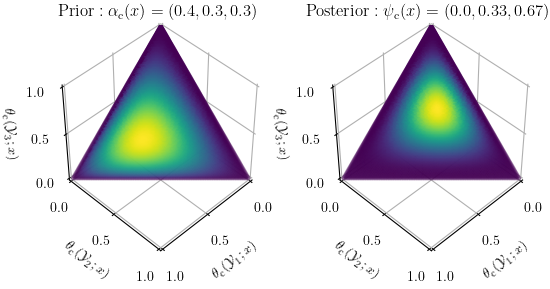
\includegraphics[width=1\linewidth]{SSP_2021/P_theta_post.png}
\caption{Model prior $\prm_{\upthetac(x)}$ and posterior $\prm_{\upthetac(x) | \uppsim(x),\uppsic(x)}$}
\label{fig:P_theta_post_tilde}
\end{figure}


%PGR: convex trends commented. cut?

%The last representation views the distribution as a convex combination of two conditional distributions. The first distribution $\Prm_{\yrm | \xrm}(y | x) = \alpha(y,x) / \alpha'(x)$ is independent of the training data and based on the prior knowledge implied via the model PDF parameter; the second distribution is the conditional empirical PMF and depends solely on $\Drm$. For both, only those values $\alpha$ and $\Drm$ corresponding to the observed value of $\xrm$ influence the distribution. 
%
%The weighting factors are dependent on these values as well. For $N'(x;D) = 0$ or as $\alpha_0 \to \infty$, the PMF tends toward the conditional distribution $\Prm_{\yrm|\xrm}$, which only depends on the model parameter $\alpha$. As the number of training examples increases or as $\alpha_0 \to 0$, $\Prm_{\yrm | \xrm,\Drm}$ tends towards the empirical conditional distribution. 








\section{Regression and the Squared Error Loss}



\subsection{Optimal Estimate: Bayesian Posterior Mean}

To find the optimal Bayesian estimator, the Bayesian predictive distribution \eqref{eq:pred_Bayes_psi} is substituted into \eqref{eq:f_opt_xD} and the posterior mean in terms of the empirical statistic is
\begin{IEEEeqnarray}{rCl} \label{eq:f_opt_SE}
f^*(x;\psi) & \equiv & \gamma(x; \psim) \sum_{y \in \Ycal} \alphac(y;x) \ y \\
&& \quad + \big(1-\gamma(x; \psim)\big) \sum_{y \in \Ycal} \psic(y;x) \ y \nonumber \;.
\end{IEEEeqnarray}
%\begin{IEEEeqnarray}{rCl} \label{eq:f_opt_SE}
%f^*(\xrm;\uppsi) & \equiv & \left( 1 + \frac{N \uppsim(\xrm)}{\alpha_0 \alpham(\xrm)} \right)^{-1} \sum_{y \in \Ycal} \alphac(y;\xrm) \ y \\
%&& \quad + \left( 1 + \frac{\alpha_0 \alpham(\xrm)}{N \uppsim(\xrm)} \right)^{-1} \sum_{y \in \Ycal} \uppsic(y;\xrm) \ y \nonumber
%\end{IEEEeqnarray}
%\begin{IEEEeqnarray}{rCl} \label{eq:f_opt_SE}
%f^*(\xrm;\uppsi) & \equiv & \left(\frac{\alpha_0 \alpham(\xrm)}{\alpha_0 \alpham(\xrm) + N \uppsim(\xrm)}\right) \sum_{y \in \Ycal} \alphac(y;\xrm) \ y \\
%&& \quad + \left(\frac{N \uppsim(\xrm)}{\alpha_0 \alpham(\xrm) + N \uppsim(\xrm)}\right) \sum_{y \in \Ycal} \uppsic(y;\xrm) \ y \nonumber
%\end{IEEEeqnarray}
The optimal estimate is a convex combination of two mean values -- the first moment of the data-independent PMF $\Prm_{\yrm | \xrm} = \mu_{\upthetac(\xrm)} = \alphac(\xrm)$, and the conditional empirical mean.

The weighting factors are inherited from $\Prm_{\yrm | \xrm,\uppsi}$; thus, larger $\alpha_0 \alpham(x)$ (i.e., stronger prior information) puts more emphasis on the data-independent estimate $\mu_{\yrm|\xrm}$, and higher data volume $N \uppsim(x)$ puts emphasis on the empirical mean.





\subsection{Squared Error Risk}

%PGR: risk eq steps? comp complexity?

Substituting the Bayesian estimator \eqref{eq:f_opt_SE} into \eqref{eq:risk_cond}, transforming to the empirical statistic, and exploiting the properties from Section \ref{sec:P_psi-theta_mc}, the excess squared error risk is 
\begin{IEEEeqnarray}{rCl} \label{eq:risk_cond_SE_dir_ex}
\Rcal_{\Theta, \mathrm{ex}}(f^* ; \uptheta) & = & \Erm_{\xrm,\uppsi | \uptheta} \Big[ \big( \mu_{\yrm | \xrm,\uppsi} - \mu_{\yrm | \xrm,\uptheta} \big)^2 \Big] \\
& \equiv & \Erm_{\xrm | \upthetam}\Big[ \lambda_{\text{Bias}}(\xrm; \upthetam) \left( \mu_{\yrm | \xrm} - \mu_{\yrm | \xrm,\upthetac} \right)^2 \nonumber \\
&& \quad + \lambda_{\text{Var}}(\xrm; \upthetam) \Sigma_{\yrm | \xrm,\upthetac} \Big] \nonumber \;,
\end{IEEEeqnarray}
a conditional expectation of two weighted functions, where 
\begin{IEEEeqnarray}{rCl} \label{eq:bias}
\lambda_{\text{Bias}}(x; \upthetam) & = & \Erm_{\uppsim | \upthetam}\left[ \gamma(x; \uppsim)^2 \right] 
\end{IEEEeqnarray}
and
\begin{IEEEeqnarray}{rCl} \label{eq:var}
\lambda_{\text{Var}}(x; \upthetam) & = & \Erm_{\uppsim | \upthetam}\left[ \frac{\big( 1 - \gamma(x; \uppsim) \big)^2}{N \uppsim(x)} \right] \;.
\end{IEEEeqnarray}
%\begin{IEEEeqnarray}{rCl}
%lambda__{\text{Var}}(x) & = & \Erm_{\uppsim(x) | \upthetam(x)}\left[ \frac{N \uppsim(x)}{\big( \alpha_0 \alpham(x) + N \uppsim(x) \big)^2} \right]
%\end{IEEEeqnarray}
%and
%\begin{IEEEeqnarray}{rCl}
%lambda__{\text{Bias}}(x) & = & \Erm_{\uppsim(x) | \upthetam(x)}\left[ \left(\frac{\alpha_0 \alpham(x)}{\alpha_0 \alpham(x) + N \uppsim(x)}\right)^2 \right] \;.
%\end{IEEEeqnarray}

The first function is dependent on the squared bias between the clairvoyant estimate $\mu_{\yrm | \xrm,\upthetac}$ and the data-independent estimate $\mu_{\yrm | \xrm}$. The second function depends on $\Sigma_{\yrm | \xrm,\upthetac}$ and measures the estimator variance in excess of the minimum squared error $\Rcal_{\Theta}^*(\uptheta)$. Both functions are scaled by factors dependent on the conditional prior localizations $\alpha_0 \alpham(x)$ and on $\upthetam$ and $N$ via expectations with respect to $\Prm_{\uppsim | \upthetam}$. 
%By the aggregation property of empirical distributions, $N \uppsim(x) | \upthetam(x) \sim \Bi\big(N,\upthetam(x)\big)$ is binomially distributed. 
%Closed forms have not been found for the empirical process expectations in \eqref{eq:bias} and \eqref{eq:var}.




\subsubsection{Trends}

\begin{figure}
\centering
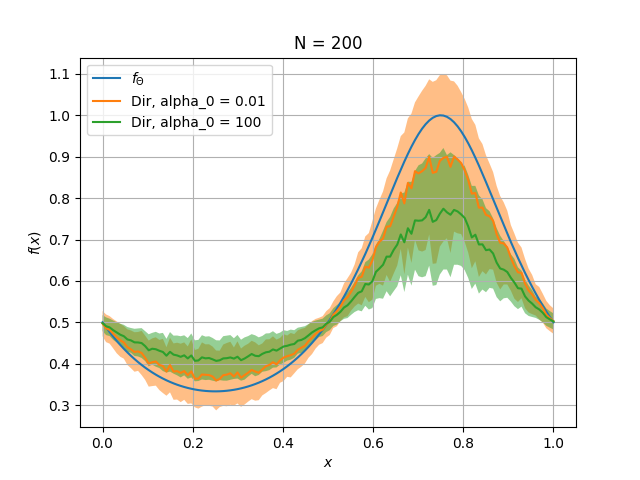
\includegraphics[width=1\linewidth]{SSP_2021/Predict_SE_biased_hard.png}
\caption{Estimator statistics, average and standard deviation}
\label{fig:Predict_SE_biased_hard}
\end{figure}

Consider the trends of the excess squared error risk \eqref{eq:risk_cond_SE_dir_ex} with training data volume $N$ and with Dirichlet prior parameterization. As $N \to \infty$, the distribution $\Prm_{\uppsim | \upthetam}$ concentrates, such that $\uppsim \inprob \upthetam$; thus, for $\upthetam(x) > 0$, the weights $\lambda_{\text{Var}}(x; \upthetam)$ and $\lambda_{\text{Bias}}(x; \upthetam)$ both tend to zero and $\Rcal_{\Theta, \mathrm{ex}}(f^* ; \uptheta) \to 0$. This desirable result is a consequence of the full support of the Dirichlet prior, which ensures the convergence of $\upthetac(x) | \uppsim(x),\uppsic(x) \inprob \uppsic(x)$ as $N \to \infty$.

Next consider the effects of the conditional prior localizations $\alpha'(x) \equiv \alpha_0 \alpham(x)$, which control a bias/variance risk trade-off. For maximal localization $\alpha'(x) \to \infty$, $\lambda_{\text{Bias}}(x; \upthetam) \to 1$ and $\lambda_{\text{Var}}(x; \upthetam) \to 0$. This is intuitive given that the estimator tends toward the data-independent solution. Conversely, for $\alpha'(x) \to 0$, $\lambda_{\text{Bias}}(x; \upthetam) \to \big( 1 - \upthetam(x) \big)^N$ and $\lambda_{\text{Var}}(x; \upthetam) \to \Erm_{\uppsim | \upthetam}\left[ \big( N \uppsim(x) \big)^{-1} \right]$. Note that the variance weight is equivalent to the first inverse moment of a positive binomial random variable \cite{stephan}.

The values $\alpha'(x)$ that minimize the excess squared error for given prior conditional distributions $\alphac(x)$ are of interest. Calculating the first derivative, it can be shown that (for $N > 0$ and $\upthetam(x) > 0$) only one stationary point exists, at 
\begin{equation} \label{eq:alpha_x_min_Rex}
\alpha'(\xrm) = \frac{\Sigma_{\yrm | \xrm,\upthetac}}{\left( \mu_{\yrm | \xrm} - \mu_{\yrm | \xrm,\upthetac} \right)^2} \;.
\end{equation}
This can readily be shown to be the global minimum.
%Evaluation of the second derivative confirms the local minimum and comparison of the local risk value to the $\alpha'(x) \to 0$ and $\alpha'(x) \to \infty$ values confirms the global minimum.

Note that the minimizing localization values $\alpha'(x)$ are inversely proportional to the squared bias of the prior conditional mean. This is sensible -- the better the match between the true and prior predictive distributions, the more confidence should be expressed. Also, low localizations are preferable when the conditional models have low variance; these models can be accurately identified by learners that emphasize the empirical mean, even with limited training data. 


\section{Examples}
To demonstrate the efficacy of Dirichlet-based regressors, consider a data model where $\Xcal$ and $\Ycal$ are 128-point discretizations of the unit interval, $\thetam$ is uniform, and $\thetac(y; \xrm) = \Bi\big(127y; 127, \mu_{\yrm | \xrm,\upthetac}\big)$; the clairvoyant estimate is $\mu_{\yrm | \xrm,\upthetac} = 1 / \big(2 + \sin(2\pi \xrm\big)$. The Dirichlet regressor is parameterized by $\alpham = \thetam$ and $\alphac(y; \xrm) = \Bi(127y; 127, \mu_{\yrm | \xrm})$, with $\mu_{\yrm | \xrm} = 0.5$. For comparison, a Bayesian linear regressor \cite{theodoridis-ML} using $\Sigma_{\yrm}=0.1$ and a Gaussian prior $\Ncal\big((0.5, 0), \Sigma_{\uptheta}\big)$ is evaluated, as well. Results are generated by averaging 50,000 iterations of a Python-based learning simulation.
%To demonstrate the efficacy of Dirichlet-based regressors, consider a data model where $\Xcal$ and $\Ycal$ are 128-point discretizations of the unit interval. The PMF $\thetam$ is uniform and $\thetac(y;x) = \Bi\big(128y; 128, \mu_{\yrm | \xrm,\uptheta}(x)\big)$, where the clairvoyant regressor is $\mu_{\yrm | \xrm,\uptheta}(x) \equiv 1 / \big(2 + \sin(2\pi x)\big)$. The Dirichlet estimator is parameterized by $\alpham = \thetam$ and $\alphac(y;x) = \Bi(128y; 128, 0.5)$. For comparison, a Bayesian linear regressor \cite{theodoridis-ML} using $\Sigma_{\yrm}=0.1$ and a Gaussian prior $\Ncal\big([0, 0.5], \Sigma_{\uptheta}\big)$ is evaluated, as well. Results were generated by averaging 50,000 iterations of a novel Python learning simulation.

Figure \ref{fig:Predict_SE_biased_hard} provides a statistical visualization (using mean and standard deviation) of the achieved regression functions. Observe that lower prior localization decreases prediction bias, but leads to more severe variance. Unlike the Bayesian linear regressor, the Dirichlet regressor uses a prior that is sufficient for approximation of complex non-linear functions.


Figure \ref{fig:Risk_cond_SE_N_biased_hard} shows the resultant expected squared error as a function of $N$. Note that only the Dirichlet regressor can achieve zero excess risk, by virtue of its full-support prior. Furthermore, with sufficient data, its performance will approach that of the clairvoyant estimator regardless of how biased the prior conditional mean $\alphac$ is, or how much confidence in $\alphac$ is indicated through the prior localization $\alpha_0$.
\begin{figure}
\centering
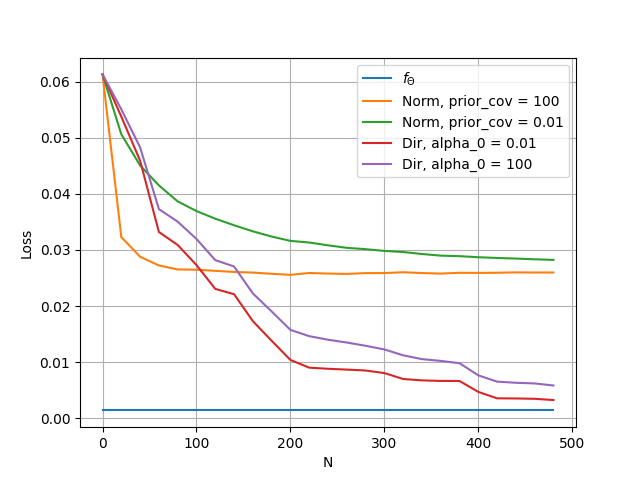
\includegraphics[width=1\linewidth]{SSP_2021/Risk_cond_SE_N_biased_hard.png}
\caption{Squared-error vs. training data volume $N$}
\label{fig:Risk_cond_SE_N_biased_hard}
\end{figure}





\section{Conclusions}

This paper has assumed a Dirichlet prior for Bayesian learning and applied the resultant predictive distribution to squared error regression. Closed-form expressions have been provided for the optimal regressor and the achieved risk. Analysis and graphical examples highlight risk trends as a function of training data volume and the Dirichlet prior localization, demonstrating a bias/variance risk trade-off.

Future work will generalize these concepts for data drawn from continuous spaces using the continuous Dirichlet process \cite{gershman}. The inherent adaptability due to the full prior support will highlight the utility of these Bayesian estimators for a wide range of regression problems; for data-limited applications, however, additional analysis is required to determine when limited-support priors are a practical necessity.




\bibliographystyle{IEEEtran}
\bibliography{../References/PhD_refs}


\end{document}

